\documentclass[twocolumn, twocolappendix]{aastex631}
\received{\today}
\shorttitle{NEOCP in Era of LSST}
\graphicspath{{figures/}}

\usepackage{lipsum}
\usepackage{physics}
\usepackage{multirow}
\usepackage{xspace}
\usepackage{natbib}
\usepackage{fontawesome5}
\usepackage{xcolor}
\usepackage{wrapfig}
\usepackage[figuresright]{rotating}

% remove indents in footnotes
\usepackage[hang,flushmargin]{footmisc} 

\newcommand{\todo}[1]{{\color{red}{[TODO: #1}]}}
\newcommand{\needcite}{{\color{magenta}{(needs citation)}}}
\newcommand{\placeholder}[1]{{\color{gray} \lipsum[#1]}}

% for shorthand/consistency
\newcommand{\dig}{\texttt{digest2}}
\newcommand{\sss}{S3M}
\newcommand{\mpco}{MPCORB}

% custom function for adding units
\makeatletter
\newcommand{\unit}[1]{%
    \,\mathrm{#1}\checknextarg}
\newcommand{\checknextarg}{\@ifnextchar\bgroup{\gobblenextarg}{}}
\newcommand{\gobblenextarg}[1]{\,\mathrm{#1}\@ifnextchar\bgroup{\gobblenextarg}{}}
\makeatother

\begin{document}

\title{The NEOCP in the Era of LSST}

% affiliations
\newcommand{\UW}{Department of Astronomy, University of Washington, Seattle, WA, 98195}

\author[0000-0001-6147-5761]{T. Wagg}
\affiliation{\UW}

\author[0000-0003-1996-9252]{M. Juric}
\affiliation{\UW}

\author{\dots more}

\correspondingauthor{Tom Wagg}
\email{tomjwagg@gmail.com}

\begin{abstract}
    \todo{}
    \placeholder{1}

    \placeholder{2}
\end{abstract}

\keywords{Near-Earth objects, Asteroids, Solar system, Small Solar System bodies, Surveys}

\section{Introduction} \label{sec:intro}
\todo{}
\placeholder{1-9}

\section{Method} \label{sec:method}
In order to make predictions for the NEOCP in the era of LSST, we make simulated observations of a catalogue of solar system objects that takes into account currently known objects. We then use the \dig{} code to calculate NEO scores for each object and use these values to make predictions for the NEOCP. In the subsections below we explain each of these steps in more details.

\subsection{Hybrid Catalogue Pipeline}\label{sec:hybrid}
Most studies that make predictions for LSST use a synthetic catalogue of solar system objects that doesn't account for prior observations \needcite{}. In reality, we have already detected more than a million objects in the solar system and this number will continue to grow until LSST comes online. This means that, current predictions of detection rates will be inflated since a fraction of ``new'' detections may already be known. Therefore, for this paper we created ``hybrid'' catalogue that combines a synthetic catalogue with all known observations, whilst keeping the population distributions relatively unchanged.

\begin{figure*}[htb]
    \centering
    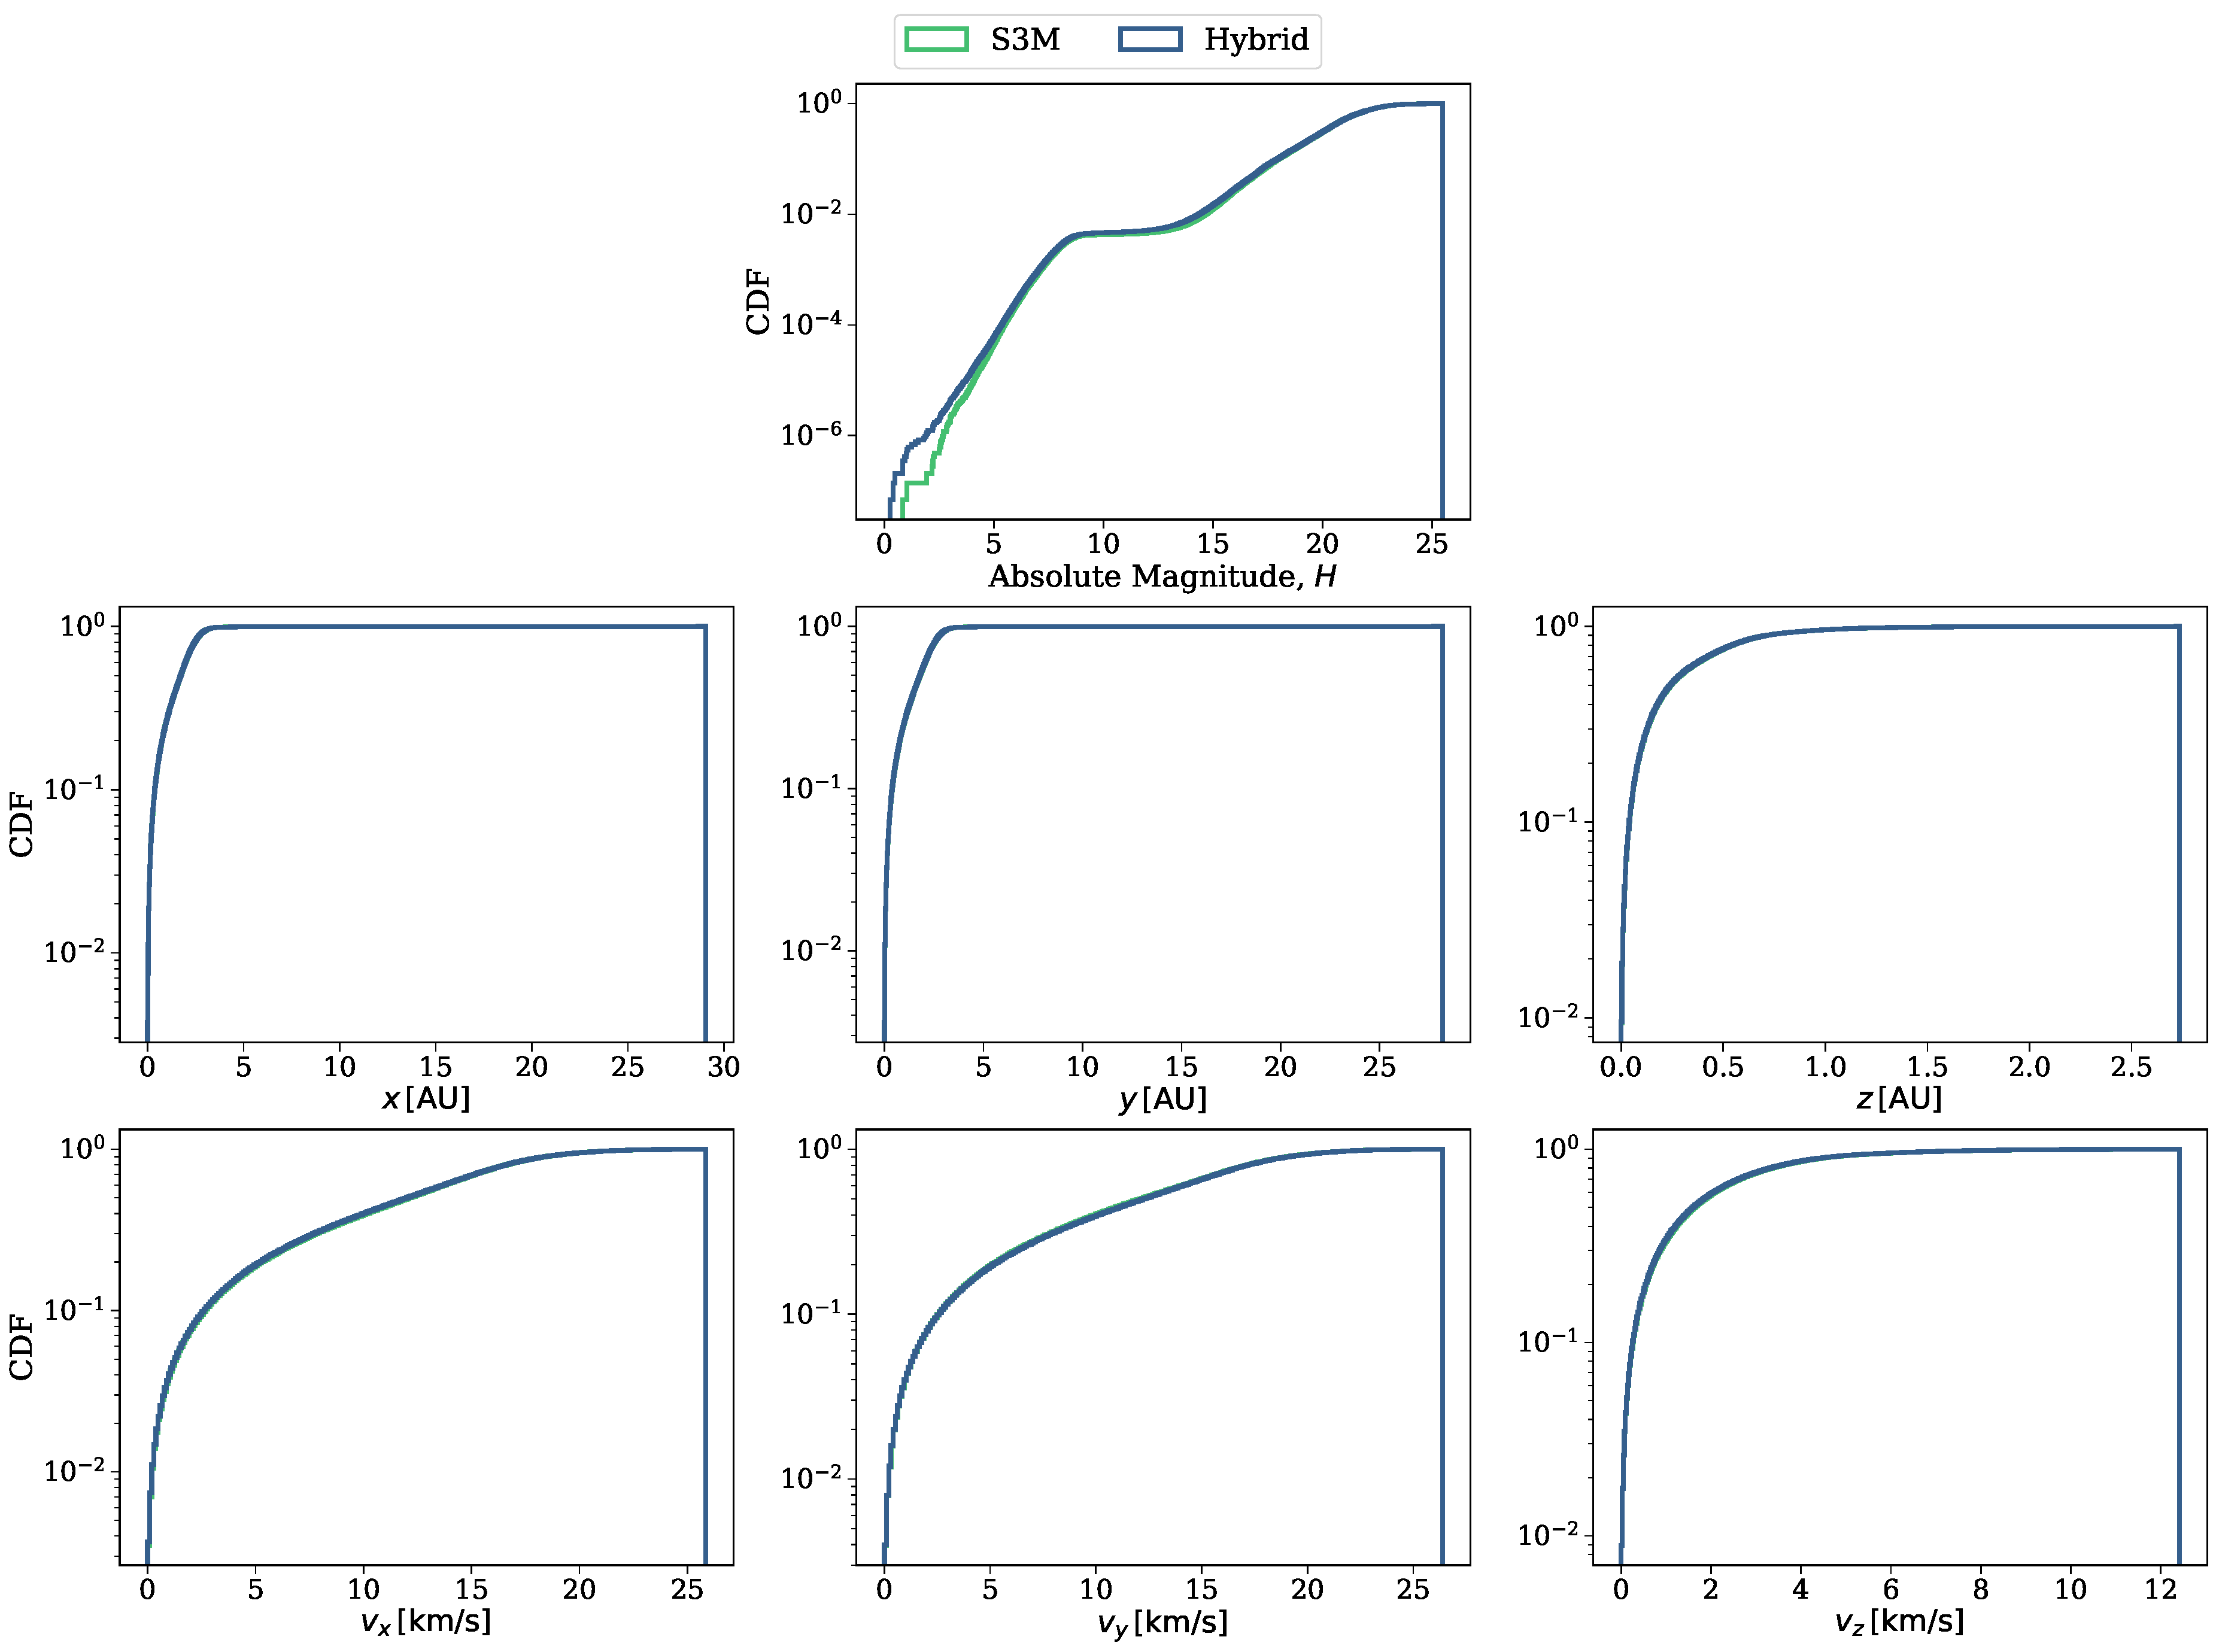
\includegraphics[width=\textwidth]{hybrid_vs_s3m_distributions.pdf}
    \caption{A comparison of the parameter distributions of S3M \citep{Grav+2011} and the hybrid catalogue we created.}
    \label{fig:hybrid_vs_s3m_dists}
\end{figure*}

We created the hybrid catalogue to be dynamic, such that we can run a single pipeline to merge in an updated version of \mpco{} as more objects are discovered in the time until LSST comes online. All code to reproduce this hybrid catalogue is open-source and available on GitHub\footnote{\url{https://github.com/dirac-institute/hybrid_sso_catalogue/tree/main/hybridcat/hybridcat}}.

\subsubsection{Data preprocessing}
For the synthetic catalogue of the solar system with we use \sss{}, the Pan-STARRS Synthetic Solar System Model \citep{Grav+2011}. We merge this synthetic catalogue with the latest version of \mpco{}\footnote{\url{https://minorplanetcenter.net//iau/MPCORB.html}}, a database of all currently known objects.

We use \texttt{OpenOrb} \citep{Granvik+2009} to convert both catalogues to Cartesian coordinates and propagate all orbits until the same date.

\subsubsection{Merging algorithm}
The general idea for the merging algorithm is to inject each object from \mpco{} into \sss{}, replacing objects that are similar to those injected. An object's similarity is determined based on its position, $\va{x}$, velocity, $\va{v}$, and absolute magnitude (size), ${H}$.

We split each catalogue into bins of absolute magnitude linearly spaced from $-2$ to $28$ and perform the merge algorithm on each bin separately. For each bin we build a K-D trees for both catalogues based on the positions ($x, y, z$) of objects. For every MPCORB object we query the S3M tree for the nearest $100$ objects up to a maximum distance of $0.1 \unit{AU}$, excluding any that have already been matched to a different real object. From these remaining nearest neighbours, we select the S3M object with the closest velocity as the matched object. If there were no remaining neighbours, either because no synthetic objects were nearby or because all nearby objects had already been matched, then we directly add this real object without replacing a synthetic one.

To complete the merging process, we compile the matched object IDs and delete them from S3M. We then add the entirety of MPCORB to the remaining catalogue, resulting in a hybrid catalogue.

\subsubsection{Assessing quality of hybrid catalogue}
It is essential that the underlying distributions of the hybrid catalogue do not differ significantly from S3M so that we still accurately reproduce the solar system. In Figure~\ref{fig:hybrid_vs_s3m_dists}, we show the distributions of the absolute magnitude and six orbital elements in both the hybrid catalogue and S3M. It is evident that the distributions are essentially identical.

As a further check, we compared MPCORB to the objects that were removed from S3M, since these should have nearly identical distributions. In Figure~\ref{fig:density_compare}, we show a comparison of the densities for the heliocentric $x$ and $y$ and it is clear that these distributions are left unchanged in the hybrid catalogue.

\subsection{Simulated Observations}

In order to investigate the effect of LSST sources on the NEOCP, we use simulated observations of the hybrid catalogue.

\todo{Should probably talk about whatever Sam did here \needcite{}}

\subsection{\dig{} Score Calculation}\label{sec:digest2_score}
The main criterion for an object to be placed on the NEOCP is for it to receive an NEO score of at least 65. This score from 0 to 100 assesses the probability that the object is an NEO and is calculated using the \dig{} code \citep{Keys+2019}. We therefore use the same code to check which of the simulated observations of the hybrid catalogue could be submitted to the NEOCP.

We use \dig{} to calculate the NEO score of each NEO and MBA in the hybrid catalogue that is observed in the first year. We apply three further cuts before considering which submissions are eligible for the NEOCP.
\begin{enumerate}
    \item \textbf{Number of observations:} We consider only objects which have at least 2 observations on a given night (though we investigate the effect of making this limit more stringent below)
    \item \textbf{Minimum arc length:} We ensure that each arc is at least 1 arcsecond in length
    \item \textbf{Maximum time separation:} We set the maximum time between observations to 90 minutes. Thus we only allow tracklets that have at least one pair of observations that occur within 90 minutes of each other
\end{enumerate}
With these cuts and the NEO scores of each object we are able to assess the load on the NEOCP from LSST.

\section{Results} \label{sec:results}
\subsection{Traffic and Purity of the NEOCP}
\begin{figure*}
    \centering
    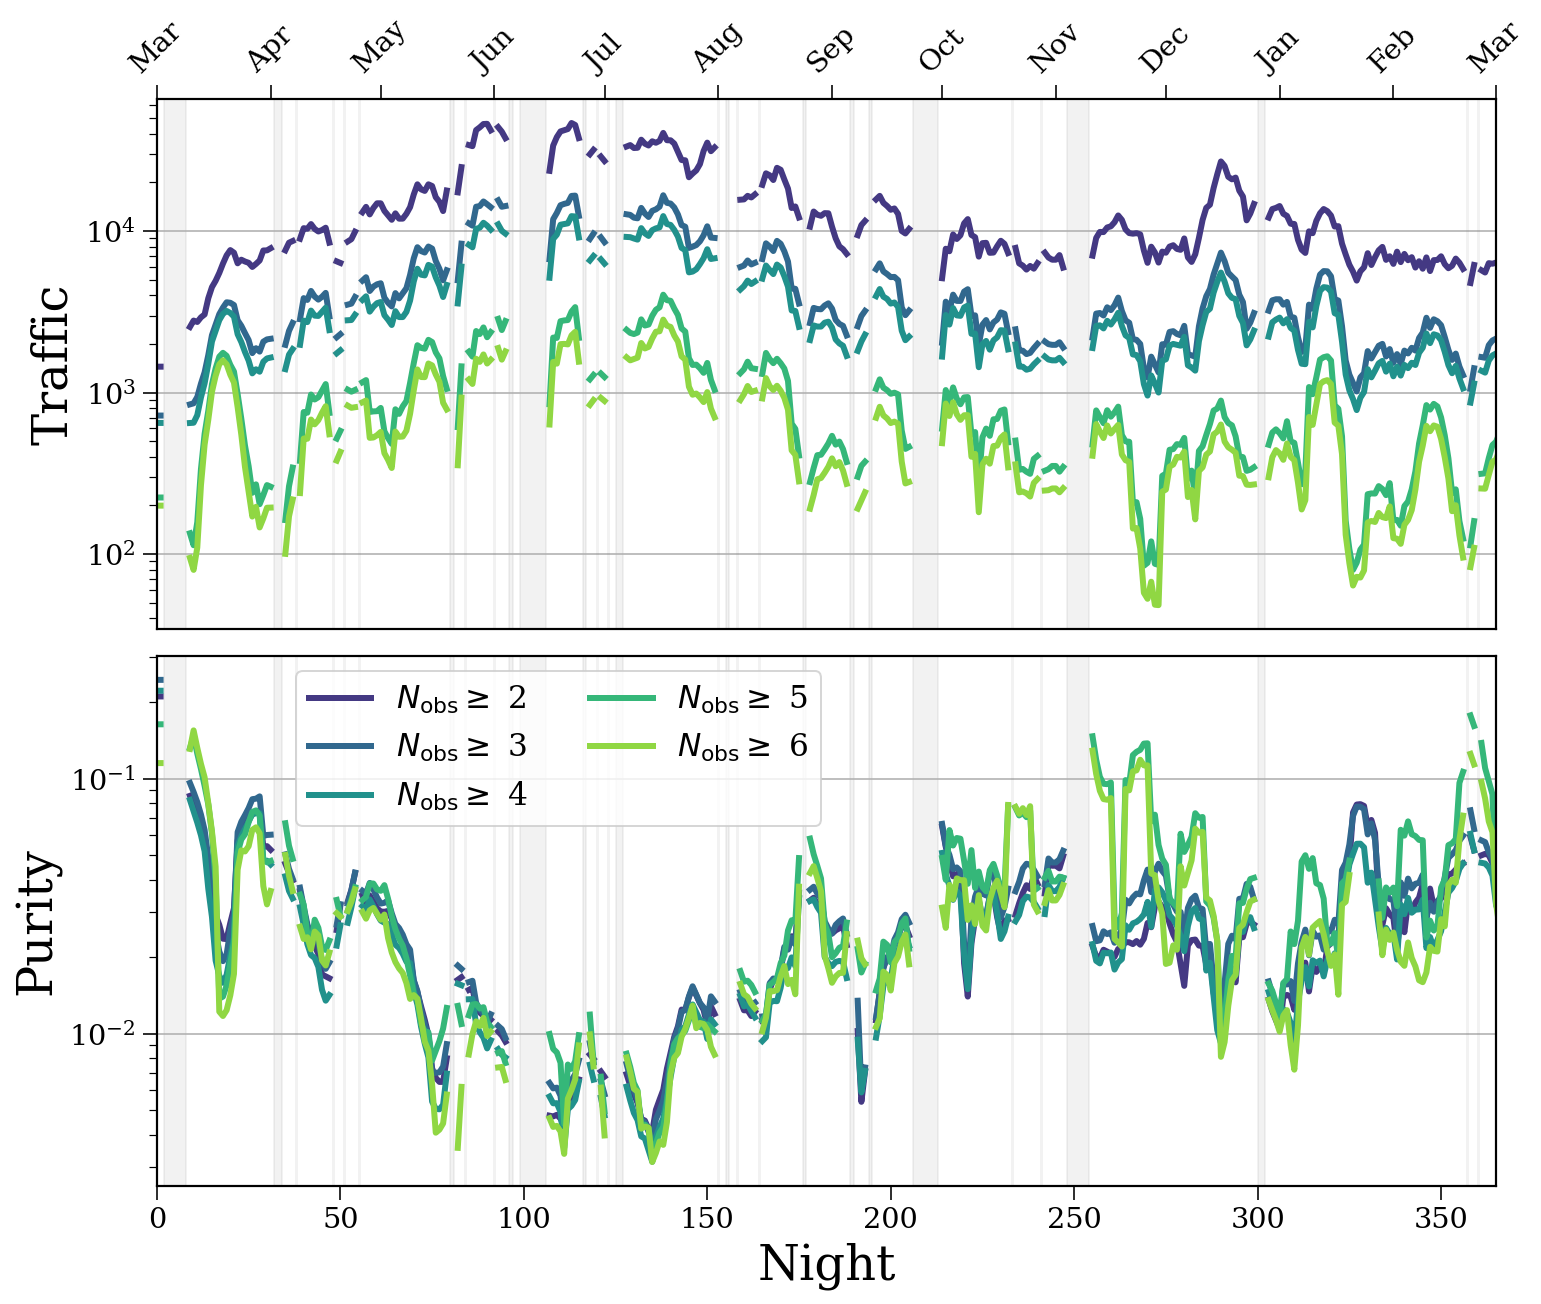
\includegraphics[width=\textwidth]{traffic_purity.png}
    \caption{Traffic (number of objects sent) and purity (fraction of objects sent that are NEOs) of the NEOCP during the first year of LSST if every observation that qualifies for submission is submitted. Each line is plotted using a rolling window of a week to smooth stochastic effects. Different lines correspond to different constraints on the number of observations for a tracklet to be submitted. Nights on which no observations were taken are highlighted with grey areas.}
    \label{fig:neocp_traffic}
\end{figure*}

In Figure~\ref{fig:neocp_traffic}, we summarise the effect of LSST submissions on the NEOCP. The top panel shows the traffic of the NEOCP, meaning the number of objects that would be submitted to the page, whilst the bottom panel shows the purity, meaning the fraction of objects submitted to the page that are actually NEOs. This plot shows the result of submitting \textit{every} qualifying observation to the NEOCP.

The current typical traffic of the NEOCP is on the order of 25 submissions per night. We show that this traffic would increase by up to 3 orders of magnitude as a result of LSST submissions. Each line corresponding to a different number of minimum nightly observations (increasing from the original choice of 2 as discussed in Section~\ref{sec:digest2_score}). Although the traffic is lower when requiring more observations, even with a minimum of 6 observations the traffic can reach several thousands of submissions per night, which is far more than the NEOCP is currently equipped to handle.

The purity of the NEOCP is also severely impacted by LSST observations, with the abundance of MBA observations polluting the page as false NEOs. For almost the entire year the page will have a purity below 10\%, meaning that only 1 in 10 objects on the page is actually an NEO. This can decrease below even 1\% and thus a lot of follow up time would be wasted in looking at MBAs masquerading as NEOs.

There are two periodic effects that can be noted in both the traffic and the purity panels. There is a clear seasonal variation over the year as the ecliptic plane moves through the sky. LSST observes from the southern hemisphere and thus in first half of the year when the ecliptic is at lower declinations, more MBAs will be observed. This both increases the traffic and decreases the purity of the NEOCP. In addition to this long term variation, there are also shorter term variations that are most clearly seen in the purity panel. On day 17 and approximately every 30 days after this there is a periodic decrease in the purity of the page. This coincides with the occurrence of a full moon, since LSST has to observe a different part of the sky during this time and this leads to more MBA detections and thus lower purity.

\todo{Check that I explained both of these effects correctly (particularly the moon one)}

\begin{figure*}
    \centering
    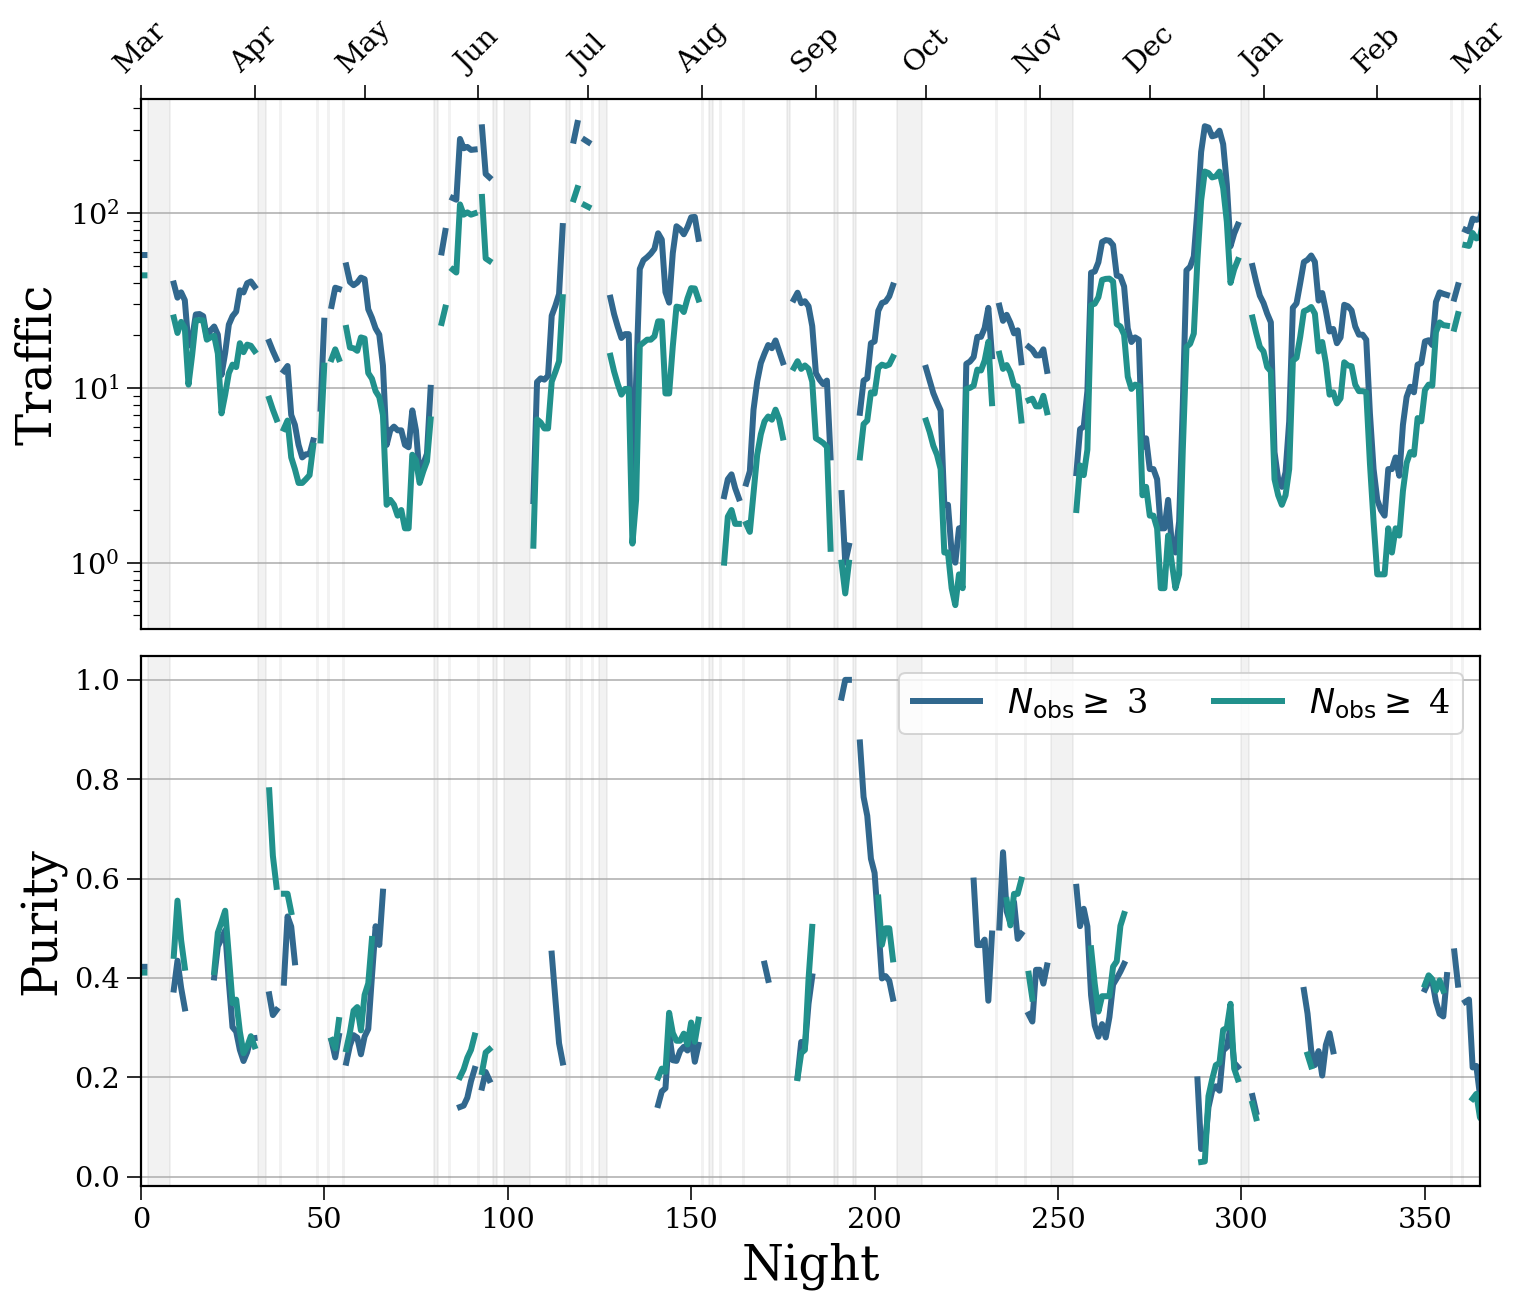
\includegraphics[width=\textwidth]{traffic_purity_unfindable.png}
    \caption{As Figure~\ref{fig:neocp_traffic}, but only including objects that would not be detected by LSST alone. Note the y-scale of the lower panel is now linear.}
    \label{fig:neocp_traffic_unfindable}
\end{figure*}

Overall, it is clear that if we proceed in the same manner as is currently recommended that the NEOCP will not be able to handle the load. We now consider how we could proceed differently.

\subsection{NEOCP without LSST Detections}\label{sec:no_LSST_detections}

LSST will be able to detect and characterise many potential NEOs without any external input. This means that many of the objects submitted to the NEOCP will actual result in wasted follow up time by the community. We assess the magnitude of this effect using the python package \texttt{difi}\footnote{\url{https://github.com/moeyensj/difi}}. This package calculates which objects are detected by LSST, where a detection is defined as occurring when the same object is observed on at least 3 separate nights, each with at least 2 observations separated by at most 90 minutes.

In Figure~\ref{fig:neocp_traffic_unfindable}, we repeat Figure~\ref{fig:neocp_traffic} but now only including objects that would not be detected by LSST alone. This represents a best case scenario in which we had foreknowledge of which observed objects would be detected. In this scenario we see that the traffic from LSST rarely exceeds more than 100 objects and is often only a handful. Similarly the purity is much higher, with an average of around 25\%. We conclude that if we were to know whether an object would be detected by LSST, the load on the NEOCP would remain at manageable levels.

\subsection{Estimating LSST Detection Probability}
We now propose a method of \textit{predicting} whether an observed object will be detected by LSST in order to emulate the best case scenario described in Section~\ref{sec:no_LSST_detections}.

For an object to be detected by LSST, it must be observed at least twice on at least three separate nights. Therefore, one can predict whether an object will be detected simply by whether it will be in LSST's field of view on the following night - if it will pass out of the field of view by the next night then it will not be detected by LSST and should be submitted to the NEOCP.

In order to determine the location of an object on the following night one needs to know its orbit. Each object on a given night consists of at least two observations
\begin{equation}
    O = \{ \alpha, \delta, t \}
\end{equation}
where $\alpha$ is the right ascension, $\delta$ is the declination and $t$ is the time of observation. One can then determine the proper motion of the object on the sky, ($\dot{\alpha}$, $\dot{\delta}$), by calculating the change in position over time between the two observations. This determines 4 and the 6 orbital elements, but the distance, $D$ and radial velocity, $\dot{D}$ of the object are unconstrained.

We draw a sample of $D$ uniformly in log-space between $0.1$-$100 \unit{AU}$ and a sample of $\dot{D}$ uniformly between $-50$-$50 \unit{km}{s^{-1}}$ to create a grid of $(D, \dot{D})$. Combining these with the measured $(\alpha, \delta, \dot{\alpha}, \dot{\delta})$ values (with some scatter to account for the detector uncertainty), we create a series of possible variant orbits for the object. We adjust these orbits to account for the light travel time using \texttt{THOR} \citep{Moeyens+2021} and then propagate them until the next night using \texttt{OpenOrb} \citep{Granvik+2009}. \todo{Check through this paragraph to check we actually do this once I actually do it haha}.

We estimate the probability of the object being detected by LSST, $P({\rm detect})$, as 
\begin{equation}
    P({\rm detect}) \propto \sum_{i = 1}^{N} \sum_{j = 1}^{M} \theta_{i, j} P(D_i) P(\dot{D}_j)
\end{equation}
where $\theta_{i, j}$ is a heaviside step function that is 1 if the orbit corresponding to distance $D_i$ and radial velocity $\dot{D}_j$ results in the object remaining in the LSST field of view and 0 otherwise, $P(D_i)$ is the probability of the distance $D_i$ occurring in the hybrid catalogue and $P(\dot{D}_j)$ is the probability of the radial velocity $\dot{D}_j$ occurring in the hybrid catalogue.

\todo{Need to explain how we know where the detector is}

\todo{Demonstrate the efficiency of this method with some plots}

\todo{Maybe also add plots of the D/dot(D) distributions of HC}

\section{Discussion} \label{sec:discussion}

\todo{Some of the results may move here, unsure what else}

\section{Conclusion \& Summary} \label{sec:conclusion}

\todo{}

\begin{acknowledgements}
    Acknowledgements
\end{acknowledgements}

\software{\dig{} v0.19.2 \citep{Keys+2019}, \texttt{OpenOrb} \citep{Granvik+2009}, \texttt{difi}, \texttt{THOR} \citep{Moeyens+2021}, \texttt{astroML} \citep{VanderPlas+2012,VanderPlas+2014}, \texttt{scipy} \citep{Virtanen+2020}}

\bibliographystyle{aasjournal}
\bibliography{paper}{}

\restartappendixnumbering

\allowdisplaybreaks
\appendix
\section{Extra Figures}\label{app:extra_figs}
\begin{figure}[htb]
    \centering
    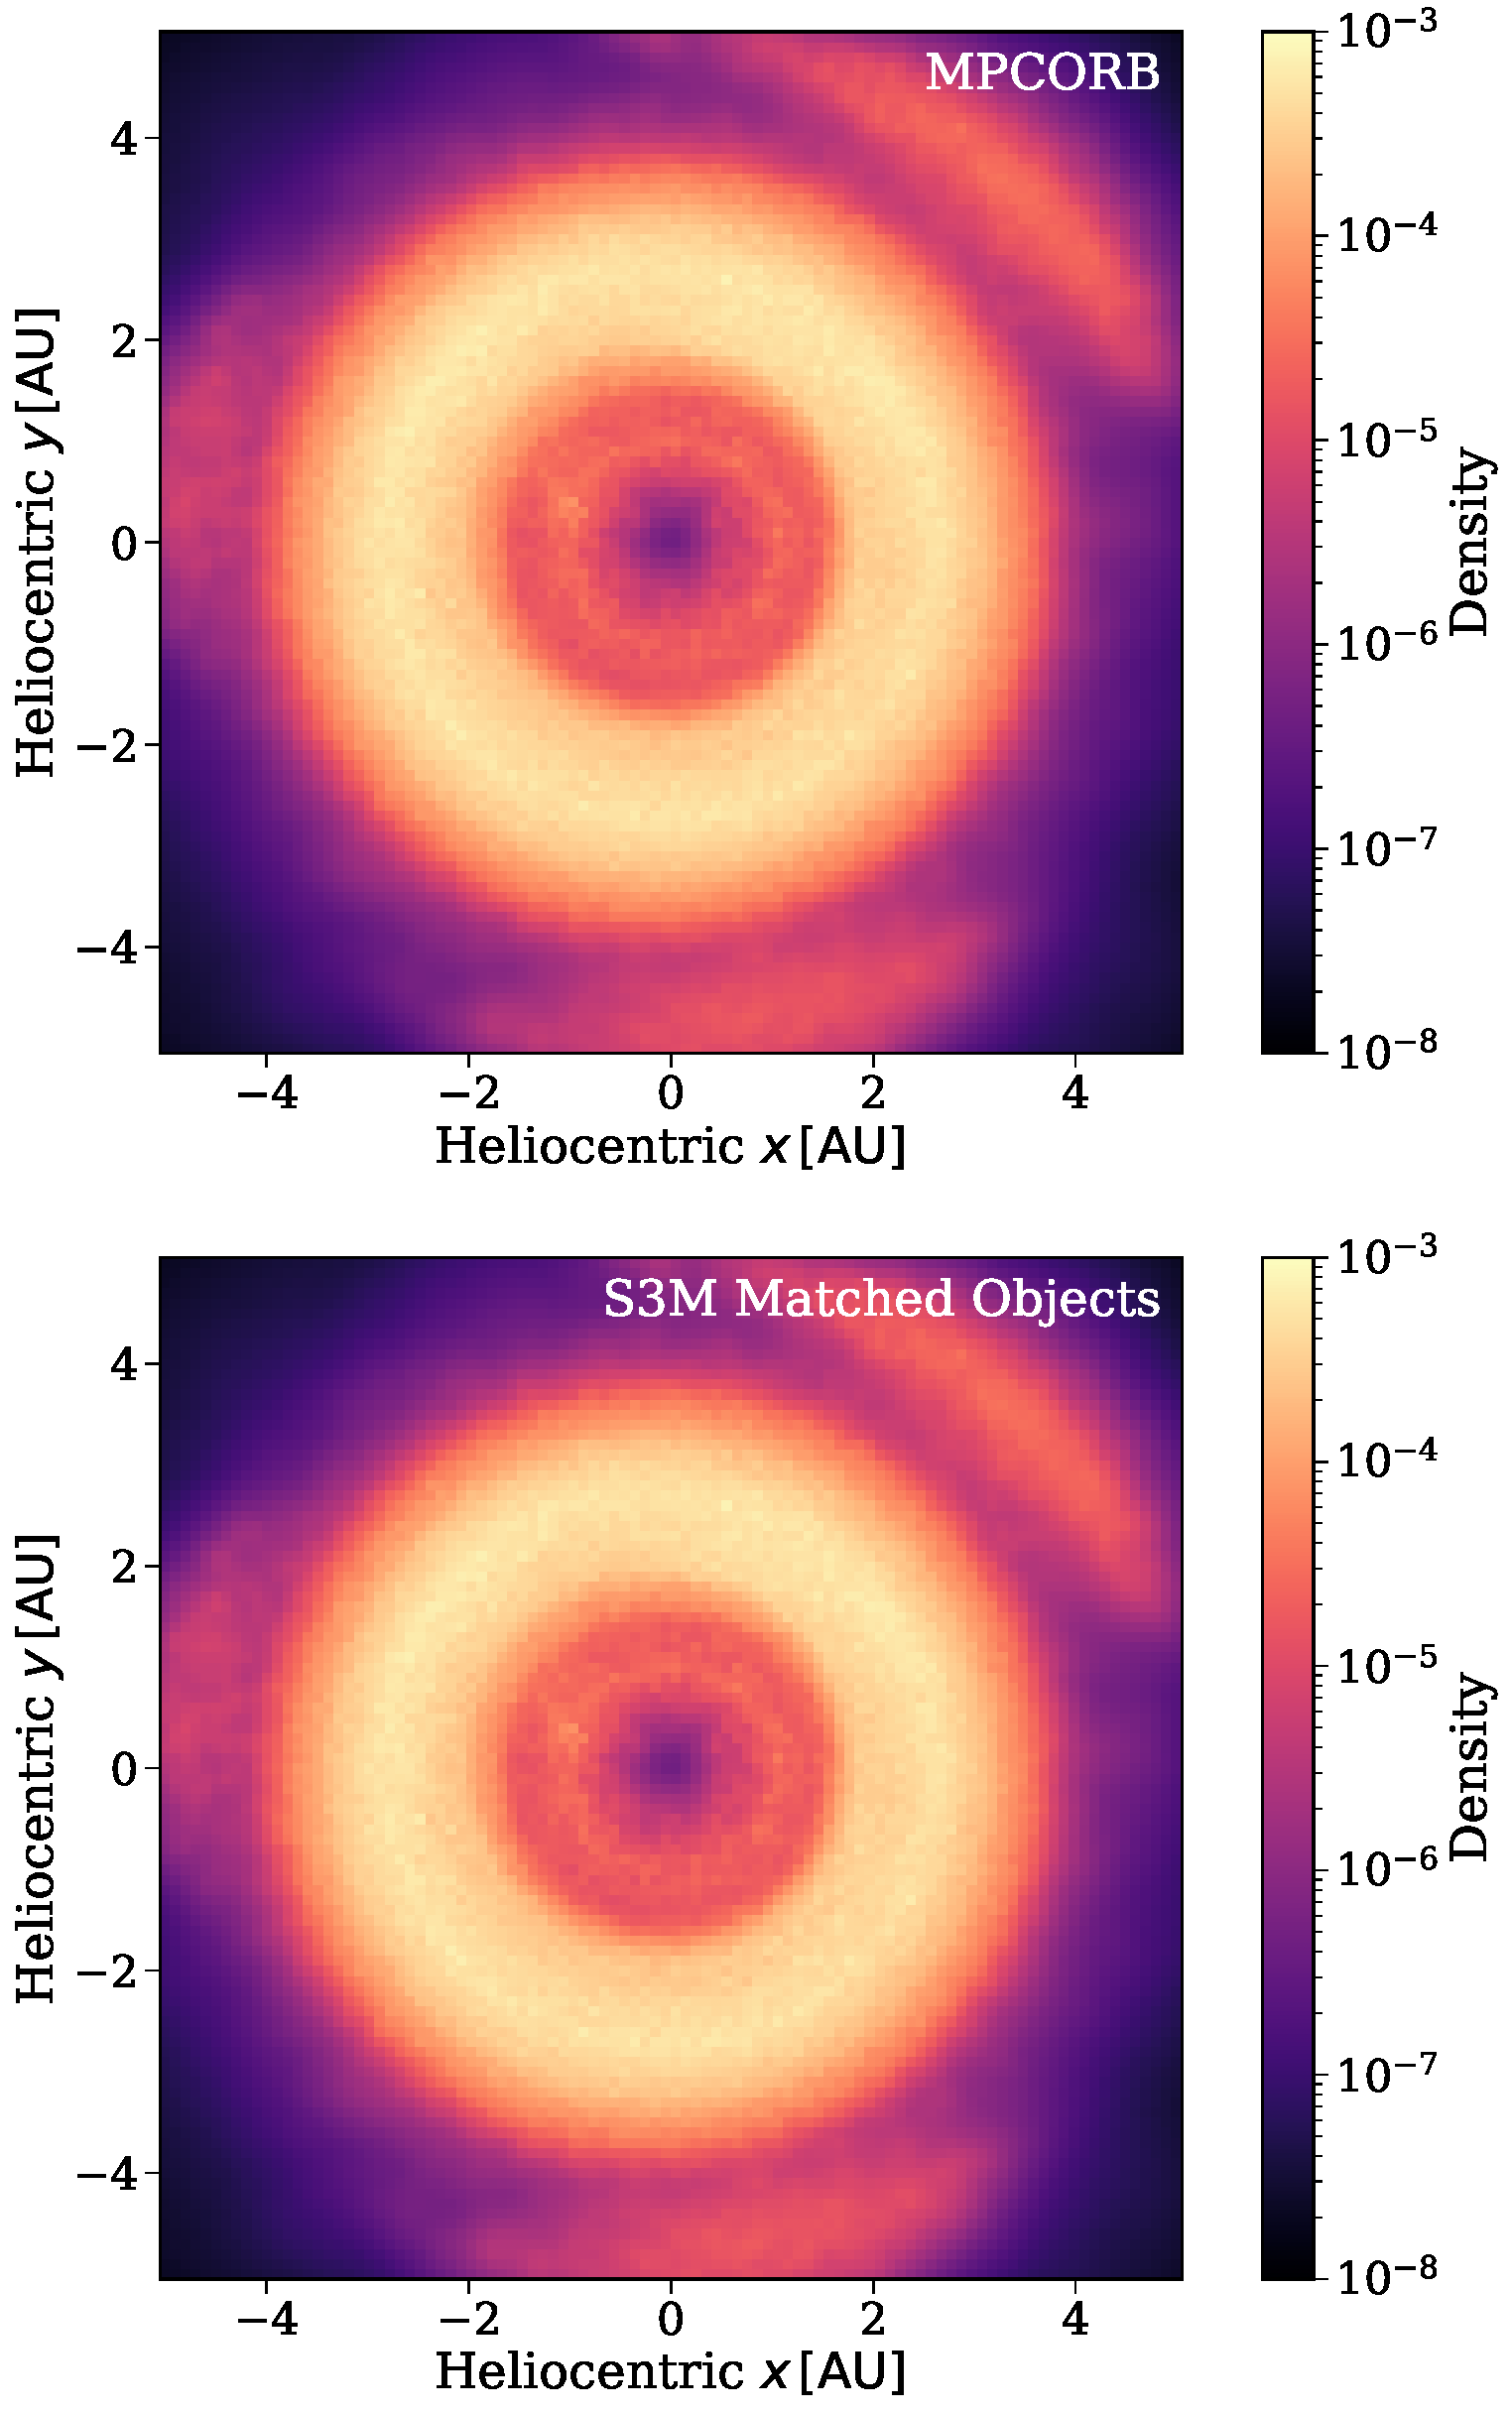
\includegraphics[width=\columnwidth]{density_comparisons.pdf}
    \caption{A comparison of the density of \mpco{} objects with those objects that were matched in \sss{} by our hybrid catalogue pipeline.}
    \label{fig:density_compare}
\end{figure}
\begin{figure}[htb]
    \centering
    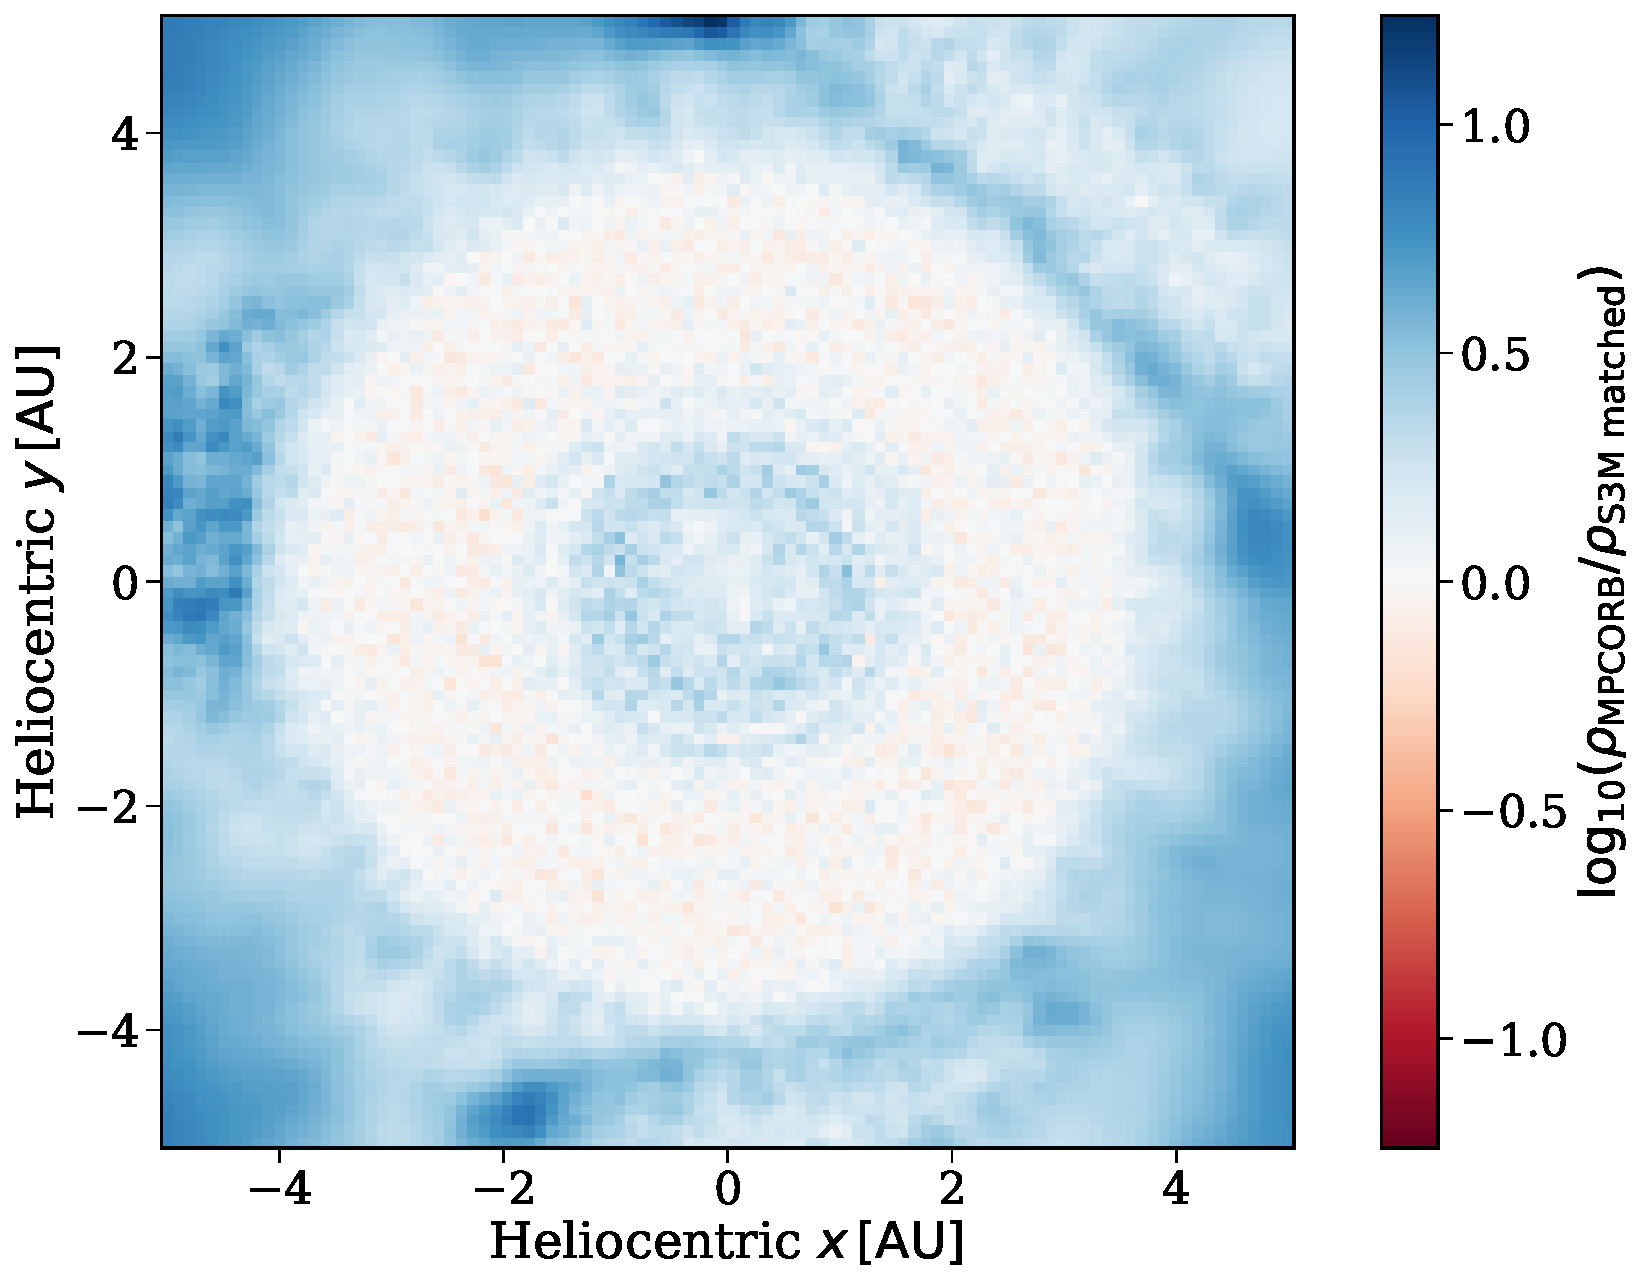
\includegraphics[width=\columnwidth]{density_residuals.pdf}
    \caption{}
    \label{fig:density_residuals}
\end{figure}

\end{document}